\documentclass[11pt]{article}

% ==== Paquetes ====
\usepackage[utf8]{inputenc}
\usepackage[spanish]{babel}
\usepackage{amsmath, amssymb, amsfonts, siunitx}
\usepackage{graphicx}
\usepackage{float}
\usepackage{minted}   % Para código con sintaxis coloreada
\usepackage{xcolor}
\usepackage{hyperref}
\usepackage{caption}
\usepackage{subcaption}
\usepackage{geometry}
\usepackage{tikz}

\geometry{margin=2.5cm}

% ==== Datos de la tarea ====
\title{IEE3584 - Comunicaciones inalámbricas \\
Tarea 3: Problema 8}
\author{Nicolás Seguel}
\date{Agosto 2025}

\begin{document}
\maketitle

\section*{Problema 8: Canal Rayleigh con Doppler}

\subsection*{a. Técnica utilizada}
Para simular el canal se utilizó el \textbf{método en el dominio de la frecuencia (FD)}. Se utiliza un espectro complejo cuya magnitud siga la densidad espectral de potencia de Clarke/Jakes:
\[
S_h(f) = \frac{1}{\pi f_D \sqrt{1-(f/f_D)^2}}, \quad |f|< f_D.
\]
Luego, aplicando una \texttt{IFFT} se obtiene la traza temporal del canal $h[n]$, que se normaliza a potencia unitaria. Este método permite reproducir fielmente la autocorrelación y la PSD del canal.

\subsection*{b. Realización del proceso de desvanecimiento}
Se generó una traza de duración $T_d=0.5\,\text{s}$, con $T_s=100\,\mu\text{s}$, 
frecuencia portadora $f_c=1.8\,\text{GHz}$ y velocidad $v=60\,\text{km/h}$.
El Doppler máximo es $f_D \approx 100$ Hz. 

En la Figura \ref{fig:fading} se observa la magnitud de la envolvente en dB.

\begin{figure}[H]
\centering
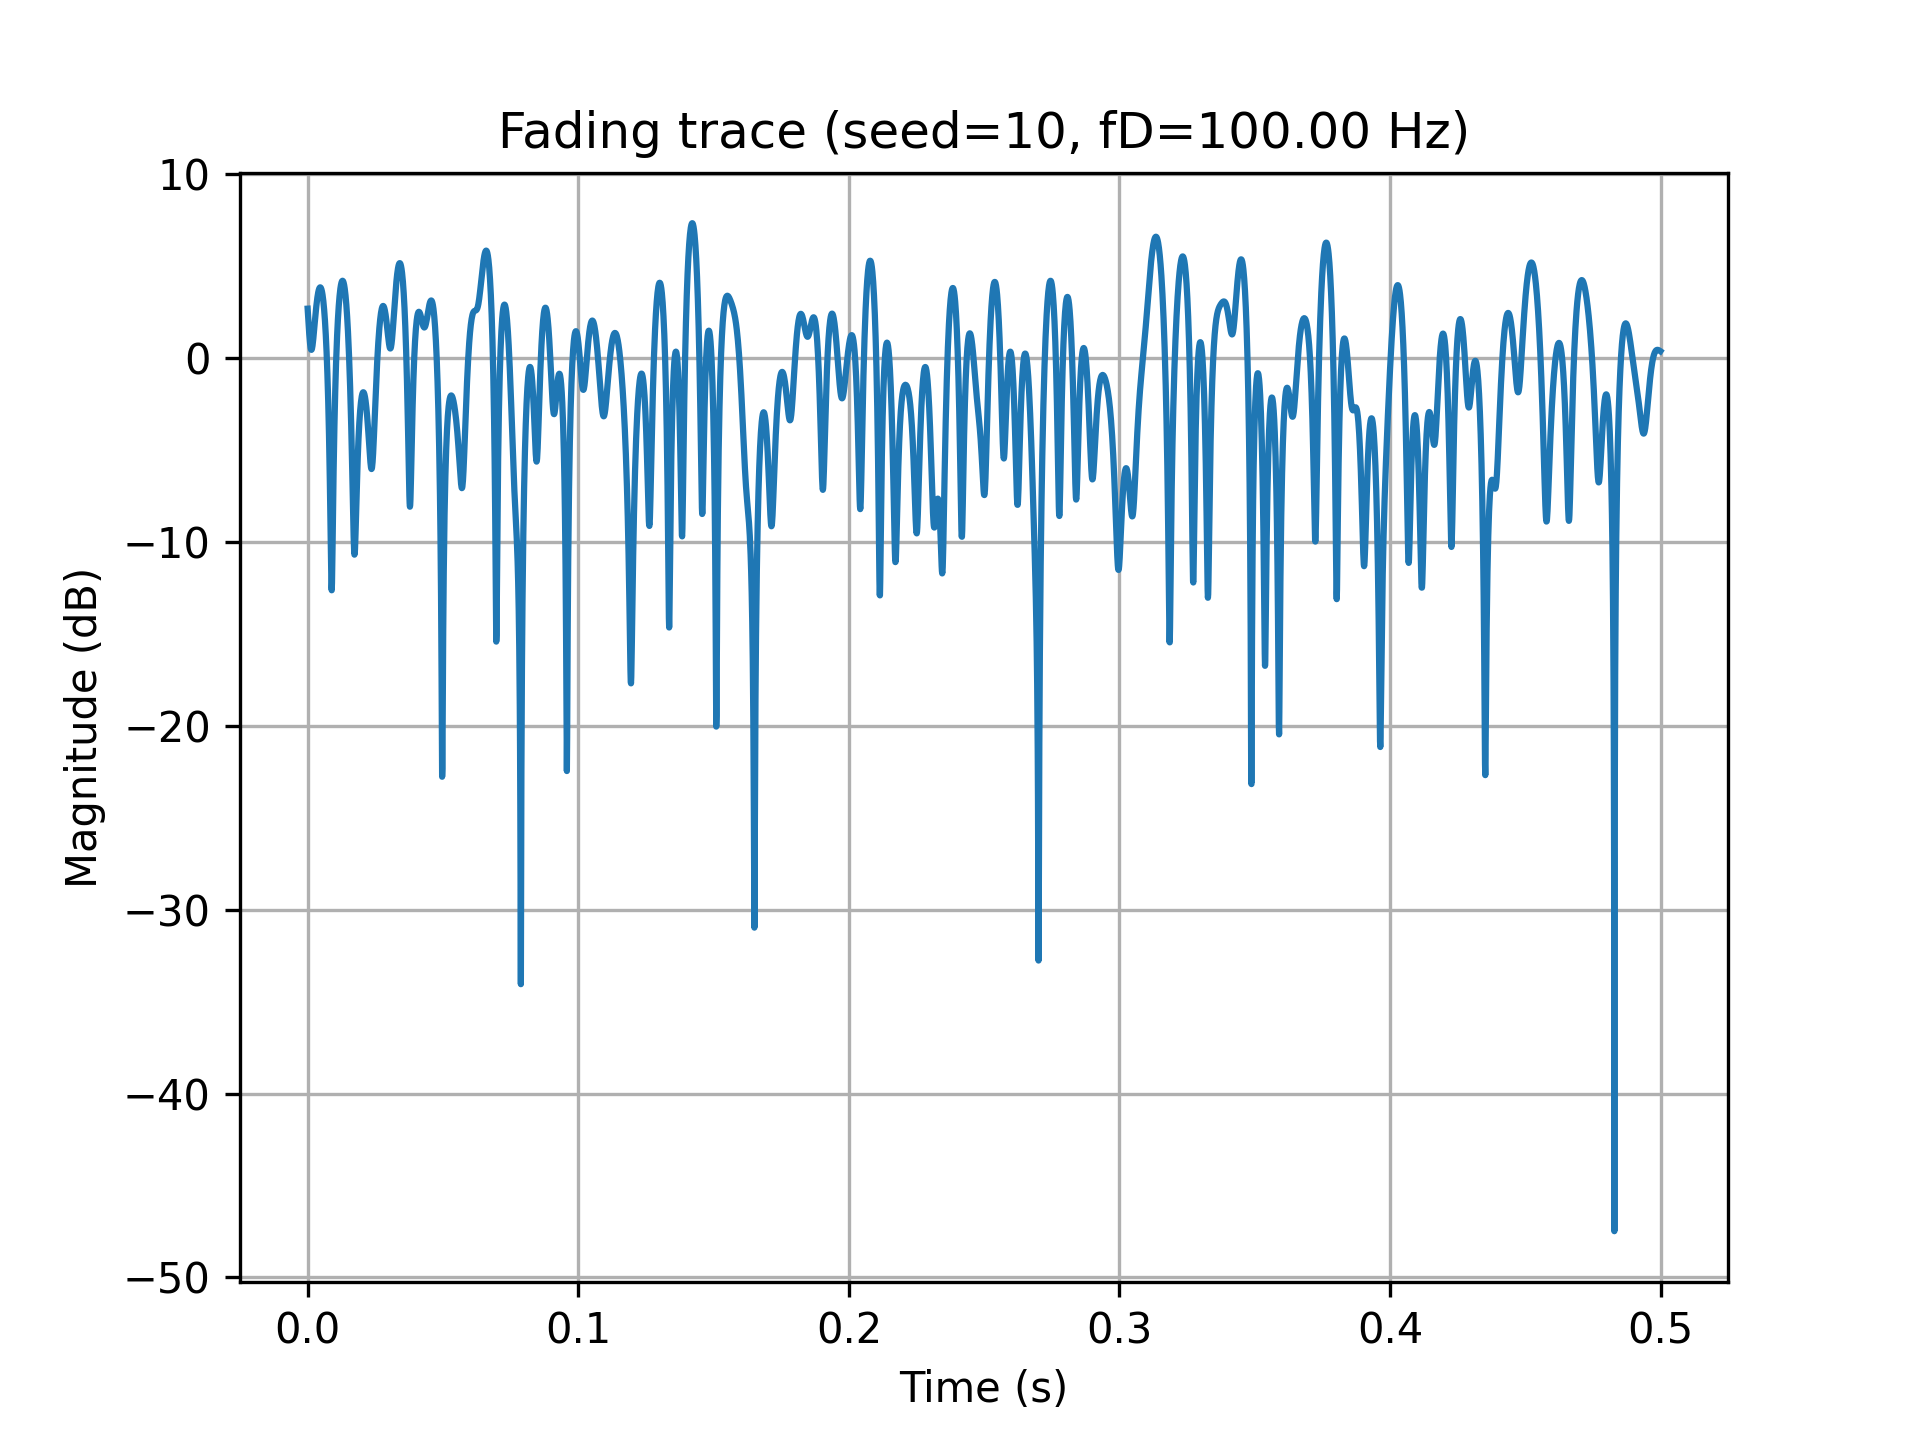
\includegraphics[width=0.8\textwidth]{fading_trace.png}
\caption{Realización temporal del canal Rayleigh en dB (seed=10).}
\label{fig:fading}
\end{figure}

\subsection*{c. Histograma y densidad de probabilidad Rayleigh}
La envolvente $r[n]=|h[n]|$ sigue una distribución Rayleigh, cuya función de densidad de probabilidad teórica es:
\[
p(r) = \frac{r}{\sigma^2} e^{-r^2/(2\sigma^2)}, \quad r\ge 0, \quad \sigma^2 = \tfrac{\lambda_p}{2}.
\]
En la Figura \ref{fig:hist} se compara el histograma de la simulación con la curva teórica.

\begin{figure}[H]
\centering
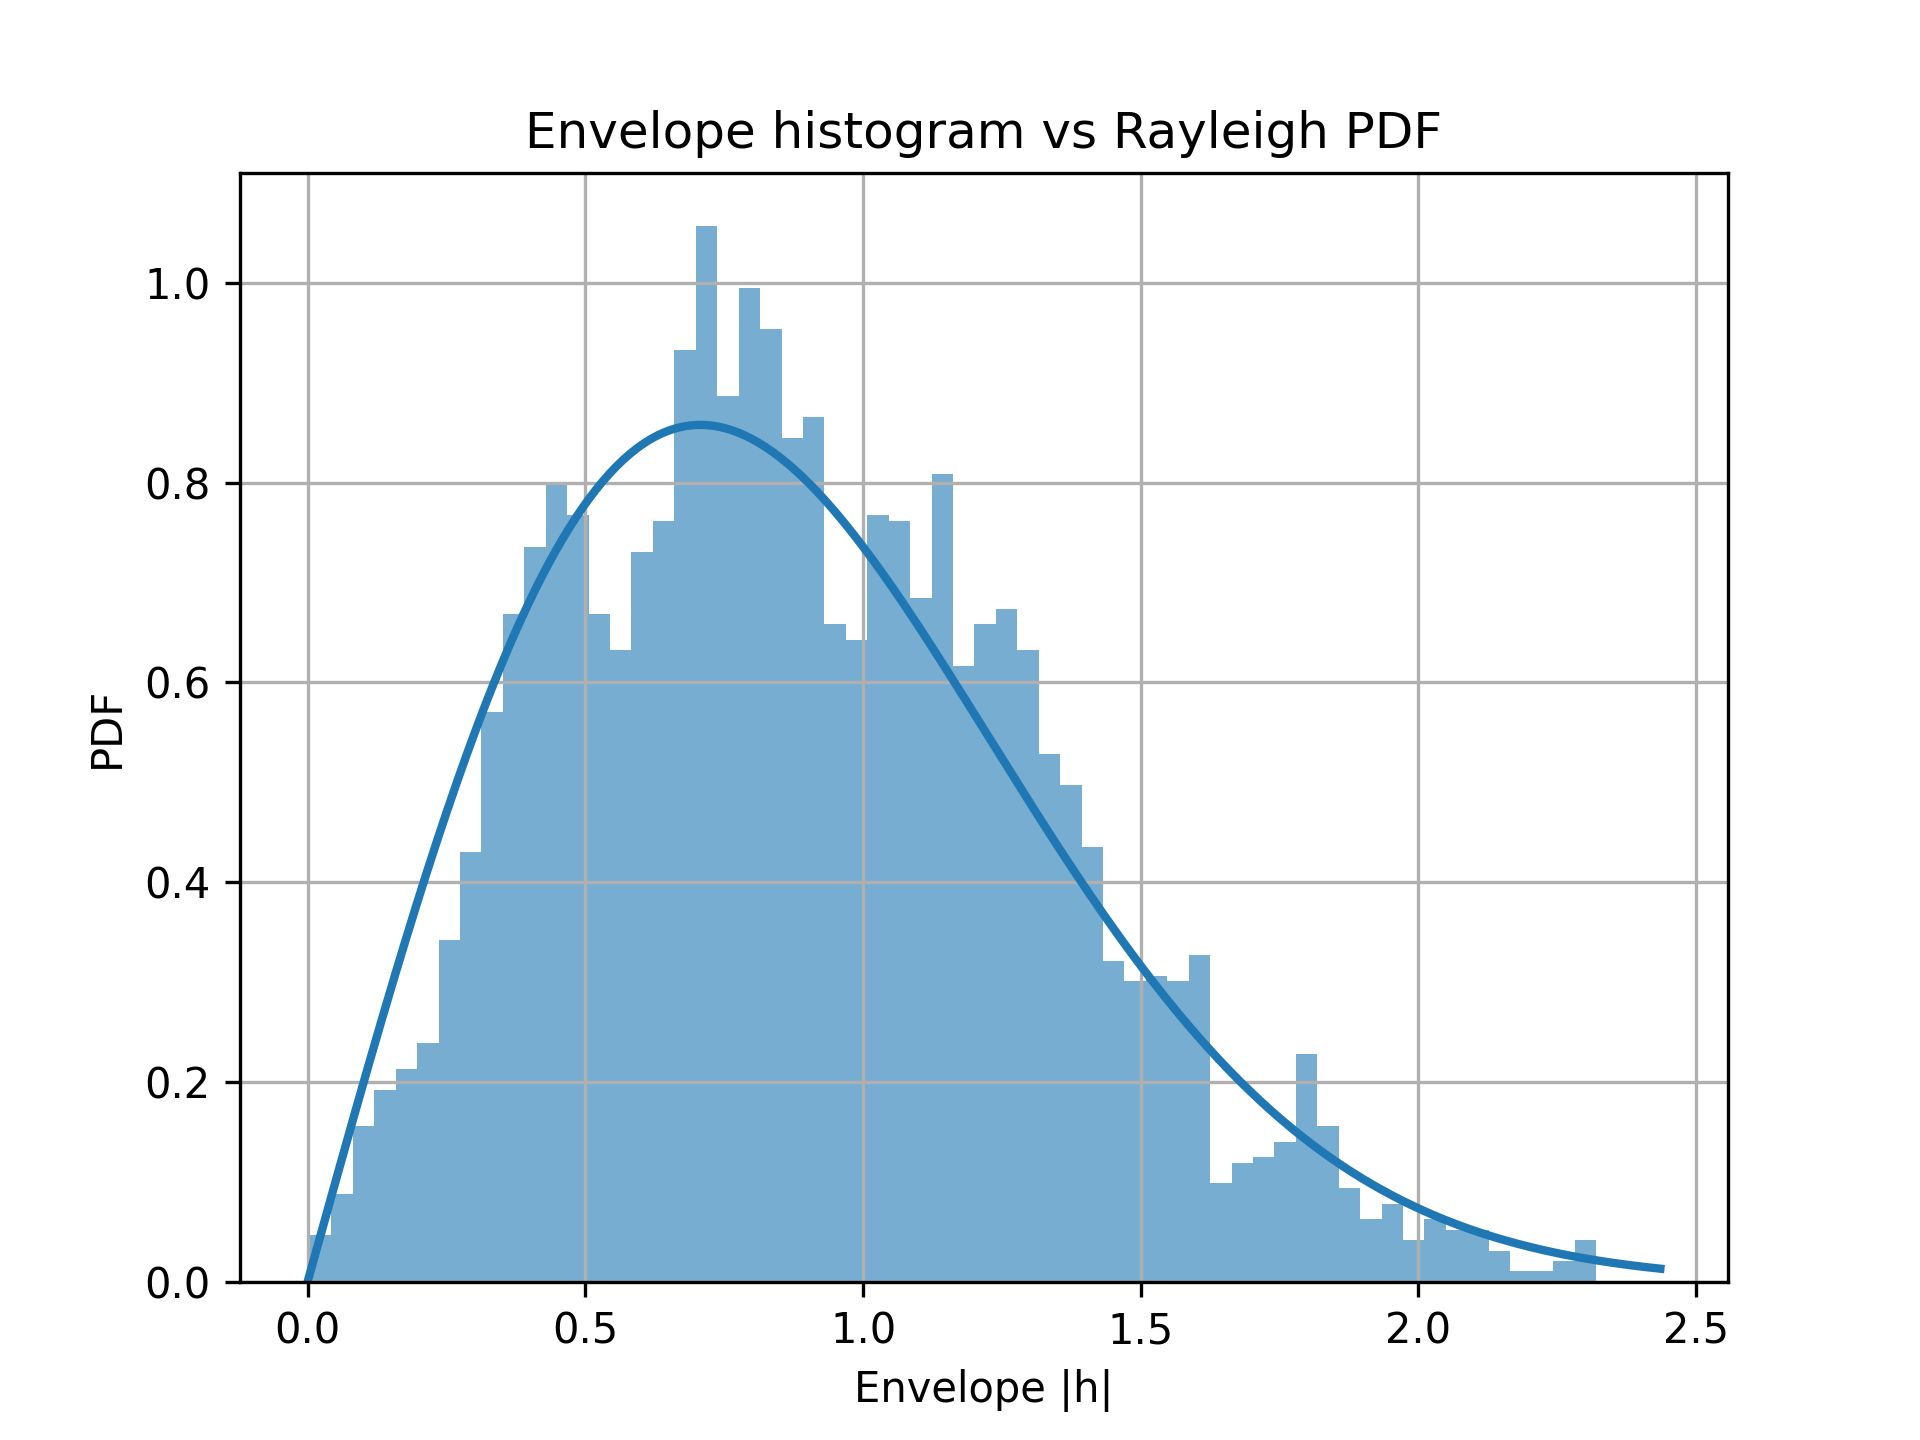
\includegraphics[width=0.8\textwidth]{histogram_rayleigh.png}
\caption{Histograma de la envolvente vs pdf Rayleigh teórica.}
\label{fig:hist}
\end{figure}

\subsection*{d. Media y valor RMS}
De la simulación:
\[
\text{Media empírica} \approx 0.9028, 
\quad \text{RMS empírico} \approx 1.0.
\]
Los valores teóricos para $\lambda_p=1$ son:
\[
E[r] = \sqrt{\tfrac{\pi}{4}} \approx 0.886, 
\quad \sqrt{E[r^2]} = 1.
\]

\subsection*{e. Densidad espectral de potencia}
La Figura \ref{fig:psd} muestra la PSD obtenida con Welch y la curva de Clarke. 
La forma de ``U invertida'' con picos en $\pm f_D$ no se logró reproducir perfectamente, principalmente por el rango de frecuencias que computa la función \texttt{welch}.

\begin{figure}[H]
\centering
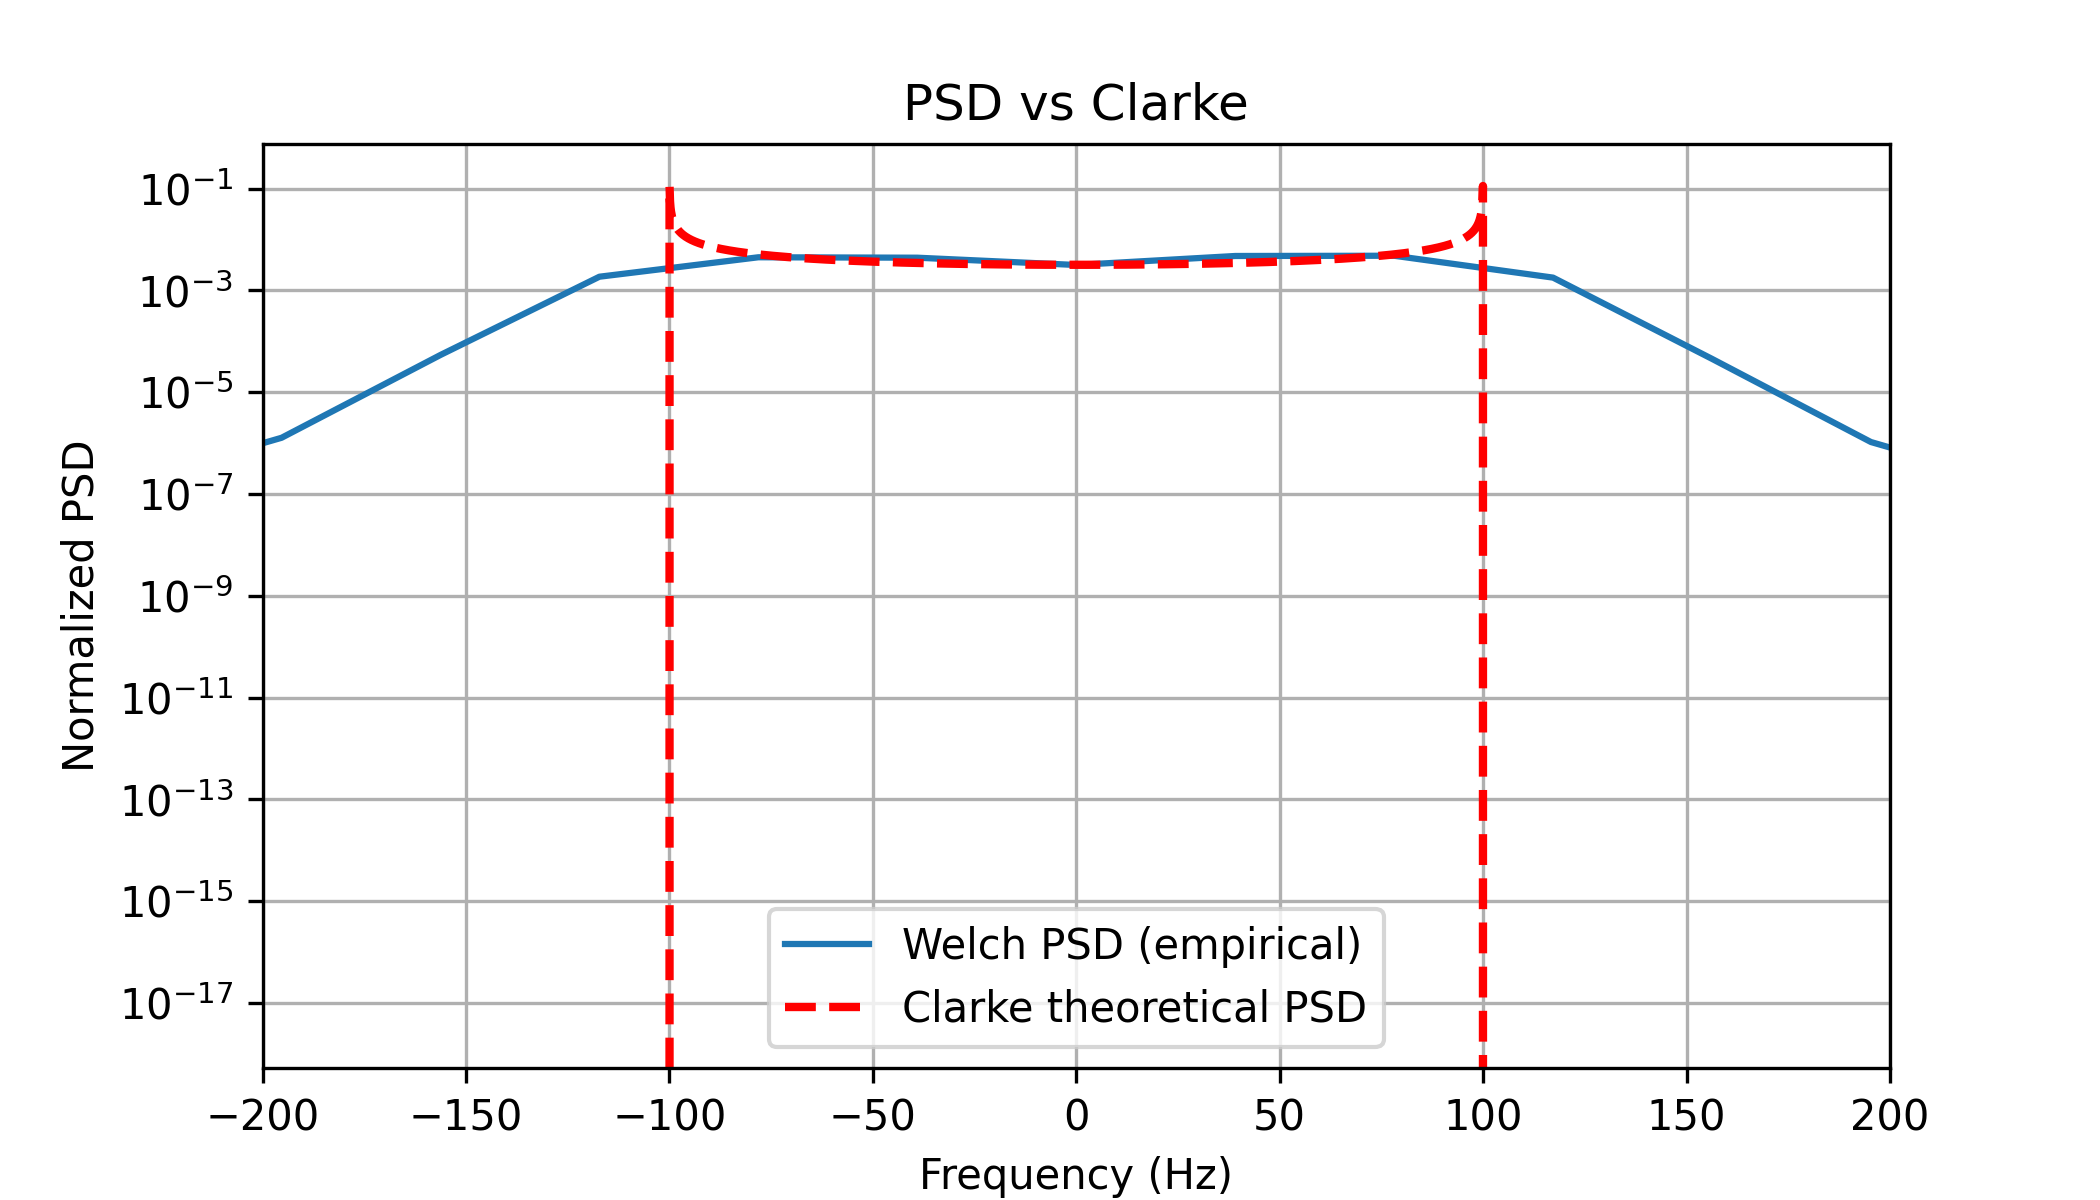
\includegraphics[width=0.8\textwidth]{psd_clarke.png}
\caption{PSD empírica (Welch) vs PSD teórica de Clarke.}
\label{fig:psd}
\end{figure}

\subsection*{f. Autocorrelación}
La autocorrelación empírica se compara con la teórica de Clarke:
\[
R_{hh}(\tau) = J_0(2\pi f_D \tau).
\]
En la Figura \ref{fig:autocorr} se observa un comportamiento similar a lo teórico, pero a una mayor frecuencia.

\begin{figure}[H]
\centering
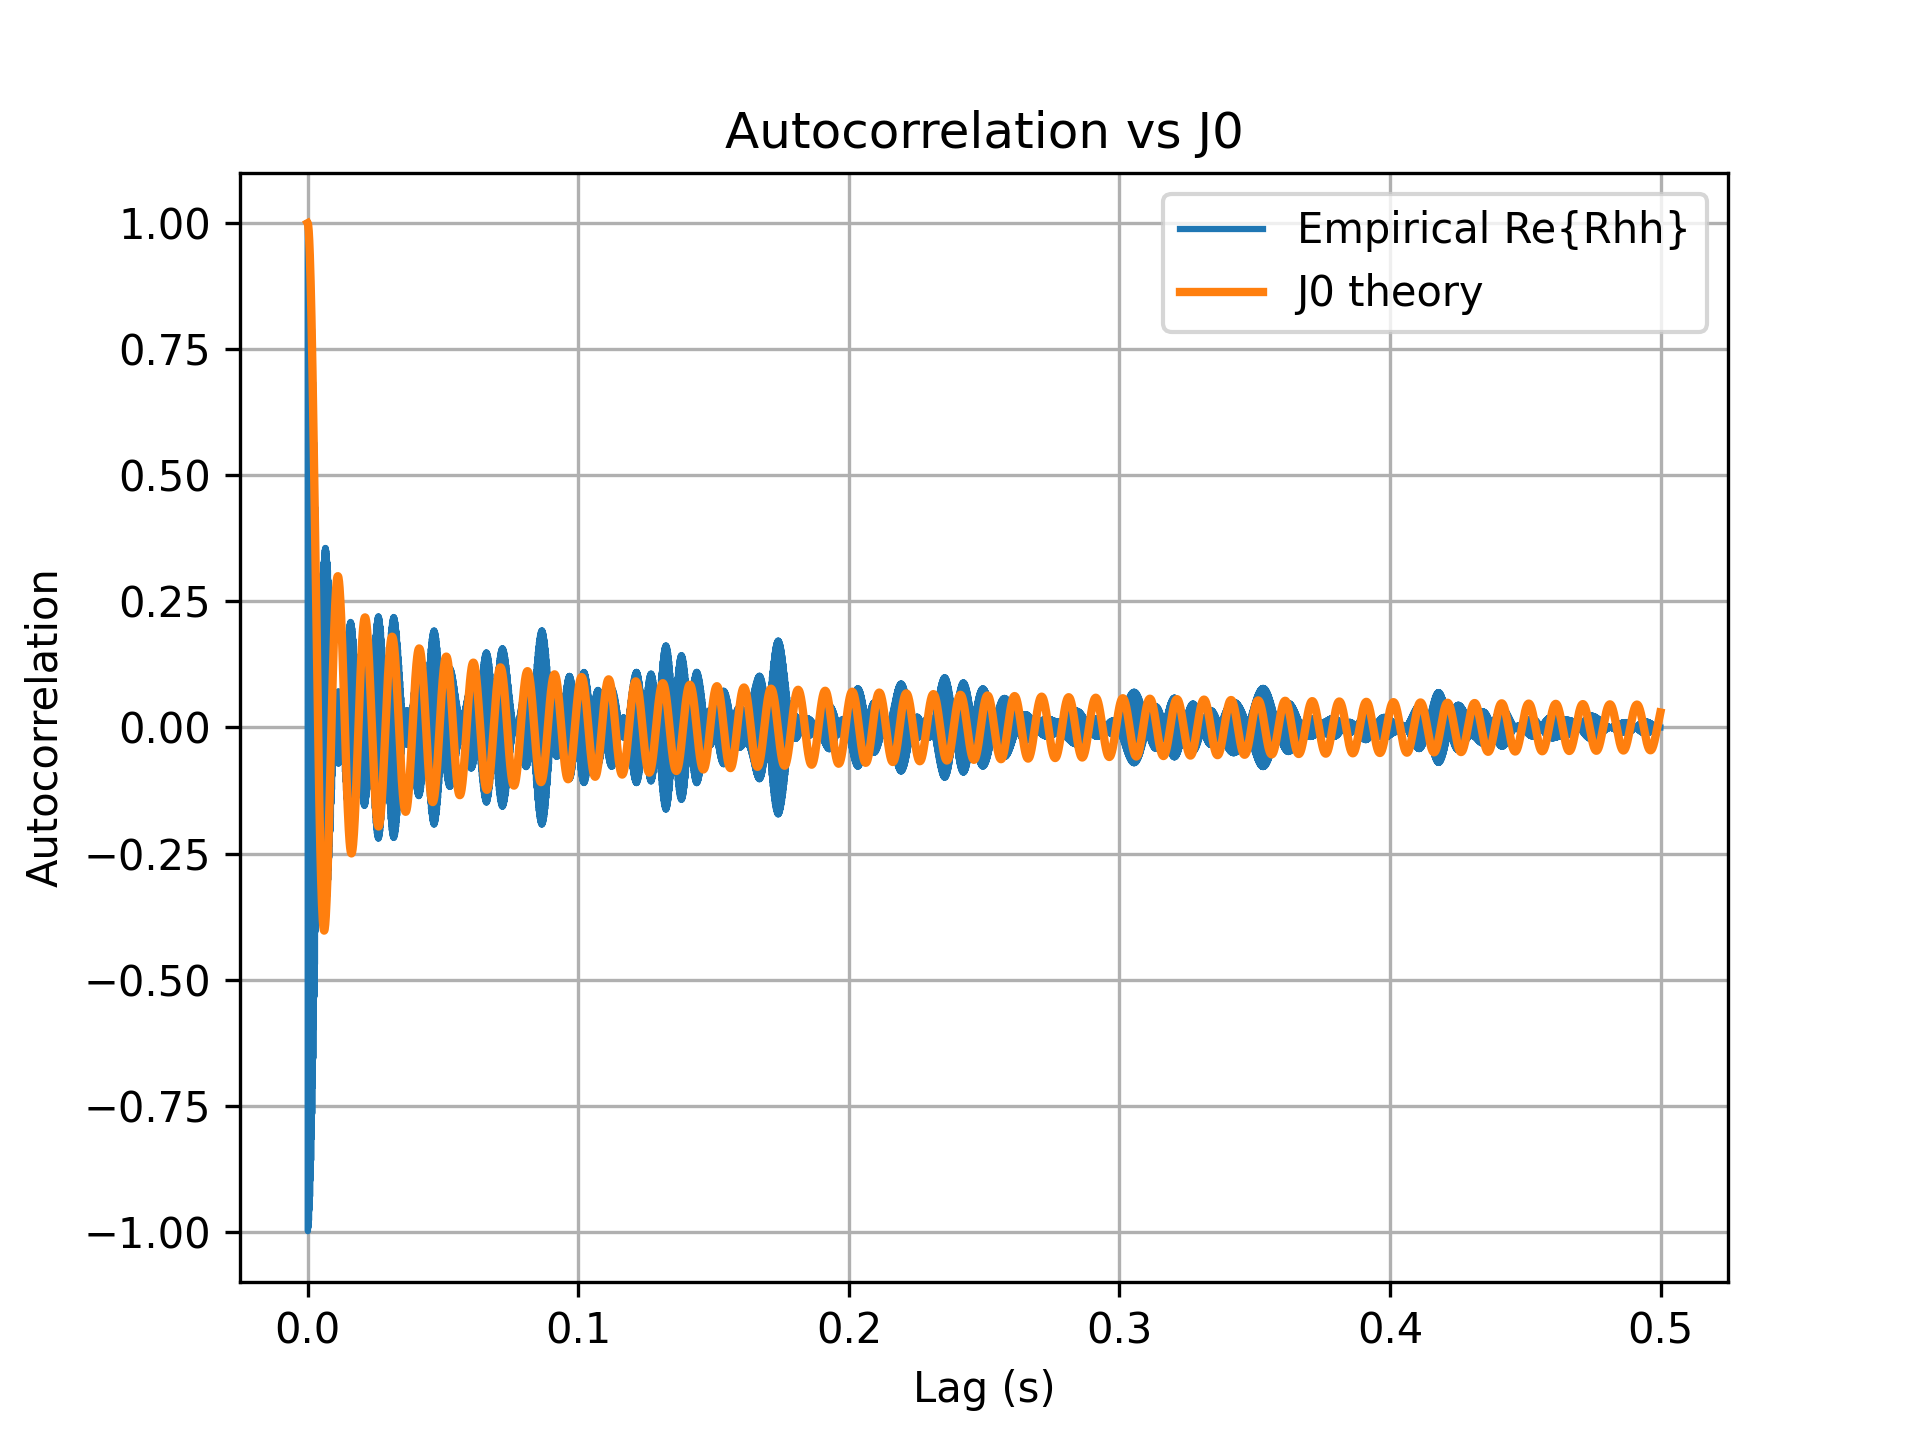
\includegraphics[width=0.8\textwidth]{autocorr_j0.png}
\caption{Autocorrelación empírica vs función de Bessel $J_0$.}
\label{fig:autocorr}
\end{figure}

\subsection*{g. LCR y AFD}
Se midieron las tasas de cruce de nivel (LCR) y la duración promedio de desvanecimiento (AFD) para umbrales de -10 dB y -20 dB respecto al RMS.

Los valores teóricos son:
\[
N_R = \sqrt{2\pi} f_D \rho e^{-\rho^2}, 
\quad T_R = \frac{e^{\rho^2}-1}{\sqrt{2\pi} f_D \rho},
\]
con $\rho = R/\sqrt{\lambda_p}$.

Los resultados empíricos y teóricos fueron bastante cercanos, siendo el AFD mayor para umbrales más altos.

\subsection*{h. Código}
El código utilizado para la simulación se incluye a continuación:

\inputminted[linenos]{python}{rayleigh_fading_simulation.py}

\end{document}
